\documentclass{article}
\usepackage{college-math-j}
\usepackage{xfrac}
\usepackage{textcomp}

%% IF YOU HAVE FONTS INSTALLED
%\usepackage{mtpro}
%\usepackage{mathtime}

\theoremstyle{theorem}
\newtheorem{theorem}{Theorem}

\theoremstyle{definition}
\newtheorem*{definition}{Definition}
\newtheorem*{remark}{Remark}

\begin{document}

\title{Computing volume via non-linear rectangular prisms}
%\author{Woodrow Wilson and Herbert Hoover} %%leave blank in initial submission to allow for double blind reviewing
%\author{ }

\maketitle

%Notes authors should leave bios out altogether.

%\begin{biog} %comment out in initial submission to allow for double blind reviewing
%\item[\biogpic{\includegraphics[width=84pt]{Woodrow_Wilson.pdf}}Woodrow Wilson] (twwilson@princeton.edu) received his PhD in history and political science from Johns Hopkins University. He held visiting positions at Cornell and Wesleyan before joining the faculty at Princeton, where he was eventually appointed president of the university.  Among his proudest accomplishments was the abolition of eating clubs at Princeton on the grounds that they were elitist.

%\item[\biogpic{\includegraphics[width=84pt]{Herbert_Hoover.pdf}}Herbert Hoover] (hchoover@stanford.edu) entered Stanford University in 1891, after failing all of the entrance exams except mathematics.  He received his BS degree in geology in 1895, spent time as a mining engineer, then was appointed by his co-author to the U.S. Food Administration and the Supreme Economic Council, where he orchestrated the greatest famine relief efforts of all time.
%\end{biog}
%This is not to say that there  This is partly, because there is no simplistic geometric interpretation for fractional calculus.  
\noindent
Bonaventura Cavalieri was a mathematician who lived in the 17th century. He made numerous contributions to the fields of optics, astronomy and geometry. 
Cavalieri was a student of Galileo. He served as a professor of mathematics at the university of Bologna from 1629 until his death in 1647. 
Galileo held Cavalieri in high esteem as is evedent from the following extract of a reference letter Galileo wrote in which he recommended Cavalieri for the chair of mathematics at Bologna: ``\emph{few, perhaps none, from 
Archimedes onwards, have investigated so deeply and have entered so far into the science of geometry}''. In 1935, a moon crater, Cavalerius, was officially named after him to commemorate his achievements and to honor his memory (see Fig ) \cite{?}. Cavalieri's most notable achievement was the publication of his 
treatise, \emph{Geometria indivisibilibus}, in which he describes the precalculus method of indivisibles. The method of indivisibles can be attributed to the ancient Greeks,
in this case Democritus and Archimedes. The method is used to compute the area and the volume of complex planar figures and solids, respectively.
It works by finding a planar figure or a solid, whose area or volume can easily be computed, which is Cavalieri congruent to a planar figure or solid whose 
area or volume is unknown. Two planar figures or solids are Cavalieri congruent if they can be decomposed into the same set of parallel ``indivisibles''. An indivisible of 
a planar figure is any cord of the planar figure. An indivisible of a solid is any planar section of a solid. Two indivisibles are equal if they are of the same length or area.
It is Cavalieri's principle that assures us that two planar figures or solids that are composed of the same set of indivisibles have equal area or volume. Cavalieri's principle 
in $\mathbb{R}^3$ is stated below without proof:

\begin{theorem}[Cavalieri's principle in $\mathbb{R}^3$]
If two solids are included between a pair of parallel planes, and if the areas of
the two sections cut by them on any plane parallel to the including planes are always
equal, then the volumes of the two solids are equal.
\end{theorem}



\noindent
Fig~\ref{??} depicts a classic rectangular prism or column as well as a \emph{non-linear rectangular prism or column}. The volumes of the two solids in Fig~\ref{??} are equal due 
to Cavalieri's principle. Note that in this article we use the non-standerdized term non-linear rectangular prism or column to refer to a solid that has a rectangular 
base and lateral edges that are non-linear and translations of one another.

\section{Cavalieri Integral}
In this section we define the Cavalieri integral \cite{ackermann12}. 


Let the region $R$ be bounded by the $x$-axis and the lines $f(x)=x$, $a(y)=1-y$ and $b(y)=4-y$. This region is shown in Fig.~\ref{fig:caval2}.\\
%\begin{figure}[htb]
%\centering
%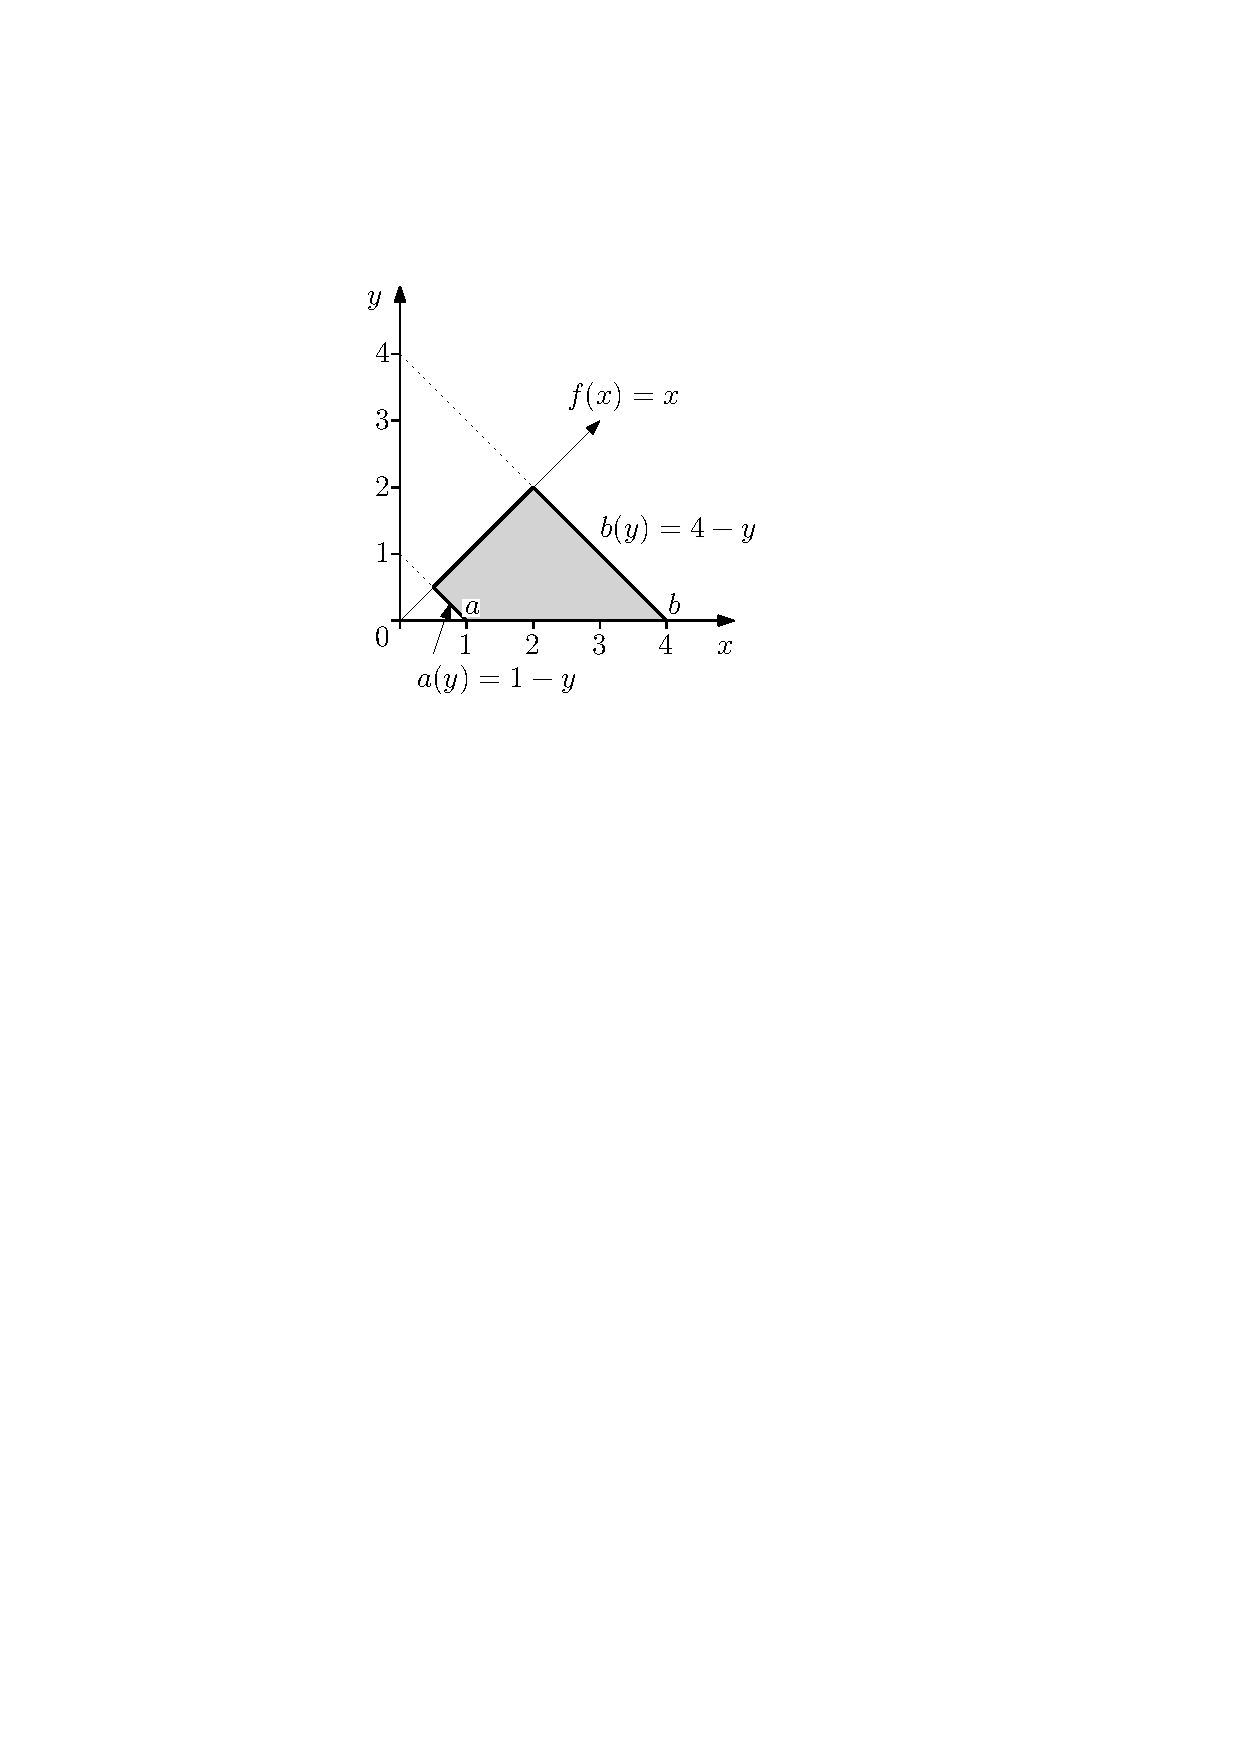
\includegraphics[width=0.3\textwidth]{fig12}
%\caption{Region bounded by the $x$-axis and the lines $f(x)=x$, $a(y)=1-y$, and $b(y)=4-y$. Reproduced from Quaestiones Mathematicae (2012) 35: 265-296 with permission \copyright~ NISC (Pty) Ltd.}
%\label{fig:ex1}
%\end{figure}


\begin{figure}[htb]
\centering
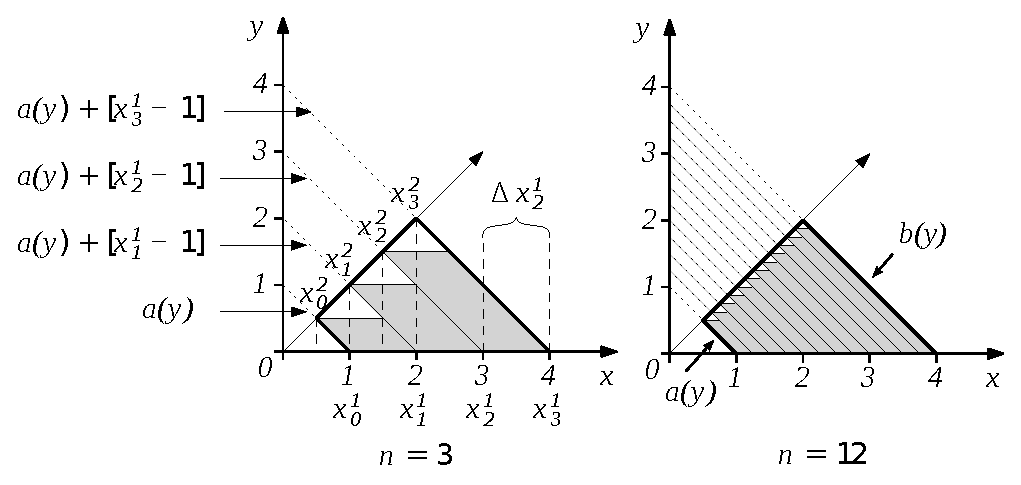
\includegraphics[width=0.75\textwidth]{fig13.eps}
\caption{Region bounded by the $x$-axis and the lines $f(x)=x$, $a(y)=1-y$, and $b(y)=4-y$. The figure also depicts the partition points $x_i^2$ as used in the Cavalieri sum (see Eq.~\eqref{eq:cav_sum}). Reproduced from Quaestiones Mathematicae (2012) 35: 265-296 with permission \copyright~ NISC (Pty) Ltd.}
\label{fig:caval2}
\end{figure}

\noindent
We can compute the area of $R$ as follows:
\begin{equation}
\int_0^2x\, dx+\int_2^44-x\, dx- \int_0^{\frac{1}{2}}x\, dx-\int_{\frac{1}{2}}^11-x\, dx = 3.75. 
\end{equation}

\noindent
However, the area of $R$ can also be determined via the Cavalieri integral:
\begin{equation}
\label{eq:caval1}
\int_{a(y)}^{b(y)}f(x)\, dx = \lim_{n\to \infty}\sum_{i=0}^{n-1} f(x_i^2)\Delta x_i^1,
\end{equation}
with $\Delta x_i^1 = x_{i+1}^1 - x_i^1$. The partition points $(x_i^1)_{i=0}^{n}$ and $(x_i^2)_{i=0}^{n}$ are depicted in Fig.~\ref{fig:caval2}. Note that 
$\Delta x_i^1$ and $f(x_i^2)$ can be interpreted as the width and the height of the $i$-th non-rectangular integration strip inscribing $R$. Their product, therefore, represents the 
area of the aformentioned integration strip. The right hand side of Equation~\eqref{eq:caval1} can therefore be interpreted as the area which 
is obtained 



We can also compute the area of $R$ by summing together non-rectangular integration strips inscribing $R$.

There, however, exists a more straightforward way do determine the area of $R$, i.e. we can sum together the area of non-rectangular integration strips inscribing $R$ instead of
having to sum together the area of multiple rectangular integration strips. Moreover, the shape of the non-rectangular integration strips we should use is determined by the function $a(y)$. We can express this notion more formally as 
follows, let $(x_i^1)_{i=0}^{n}$ denote a partition on the $x$-axis, such that $a = x_0^1 < x_1^1 < \cdots < x_n^1 = b$, and $\Delta x_i^1 = x_{i+1}^1 - x_i^1$.
We are now able to construct the following sum (the lower Cavalieri sum):
\begin{equation}
\label{eq:cav_sum}
\sum_{i=0}^{n-1} f(x_i^2)\Delta x_i^1.
\end{equation}
The partition points $(x_i^2)_{i=0}^{n}$ are depicted in Fig.~\ref{fig:caval2}. Note that Eq.~\eqref{eq:cav_sum} approximates the area of $R$. In the limit Eq.~\eqref{eq:cav_sum} approaches 
the Cavalieri integral:
\begin{equation}
\label{eq:caval1}
\int_{a(y)}^{b(y)}f(x)\, dx = \lim_{n\to \infty}\sum_{i=0}^{n-1} f(x_i^2)\Delta x_i^1.
\end{equation}
It is, however, quite hard to evaluate the above integral directly. Fortunately, it is easy to convert a Cavalieri integral into an equivalent Riemann or Riemann-Stieltjes 
integral by using the transformation functions $h$ and $g$. Expressed mathematically:
\begin{equation}
\label{eq:main_cav}
\int_{a(y)}^{b(y)}f(x)\,dx =\int_a^b f \circ h (x)\, dx = \int_{a'}^{b'} f(x) dg(x).
\end{equation}
We can calculate $g$ as follows:
\begin{equation}
g(x) = x - a\circ f(x) + a.
\end{equation}
Moreover, $h=g^{-1}$. We can now evaluate the Cavalieri integral by using its equivalent Riemann or Rieman-Stieltjes integral.
If we use its Riemann equivalent we obtain:
\begin{equation}
\int_{a(y)}^{b(y)}f(x)\, dx = \int_a^b f \circ h (x)\, dx = \dfrac{1}{2}\int_1^4x\, dx = 3.75.  
\end{equation}
If we use its Riemann-Stieltjes equivalent we obtain:
\begin{equation}
\int_{a(y)}^{b(y)}f(x)\, dx = \int_{a'}^{b'} f \, dg(x) = \int_{\frac{1}{2}}^2x\, d2x = 3.75.  
\end{equation}

\noindent
Conversely, if $g$ is known (and not $a(y)$) and $g(a') = a$ then we can calculate $a(y)$ using the following \cite{grobler19}:
\begin{equation}
\label{eq:a_y}
a(y) = f^{-1}(y) - g\circ f^{-1}(y) + g(a'). 
\end{equation}
Eq.~\eqref{eq:a_y} allows us to transform a Riemann-Stieltjes integral into an equivalent Cavalieri integral. 
Furthermore, this transformation enables us to assign a geometric interpretation to a Riemann-Stieltjes integral. The interpretation being:
it represents the area obtained by summing together the area of an infinite number of non-rectangular infinitesimals; all of them being translations of $a(y)$. Note,
$b(y) = a(y) + (b-a)$.






%One first divides a complex planar figure whose area is unknown into indivisible parallel chords. These cords are then translated 
%in such a way that the original planar figure is transformed into a planar figure whose area is easily computable. The volume of a complex solid can be computed 
%in a similar manner. 
%In this method areas of complex planar figures are computed by dividing such figures into indivisible parallel chords. One then 
%finds another planar figure whose area is known that consists of the exact same set of chords. The area of the complex planar figure is then 
 


\begin{abstract}
We presented a novel geometric interpretation of the Riemann-Liouville fractional integral. We found that a Riemann-Liouville integral can 
be thought of as the area obtained by summing together the area of an infinite number of non-rectangular infinitesimals whose shape is determined by the 
order of integration $\alpha$ and the integration limit $t$. We also showed that this geometric interpretation offers many pedagogical benefits as it is very similar
in nature to the geometric interpretation of the Riemann integral.   
\end{abstract}

\begin{thebibliography}{1}

\bibitem{ackermann12} Ackermann,~E.~R, Grobler,~T.~L., Kleynhans,~W., Olivier,~J.~C., Salmon,~B.~P, van Zyl,~A.~J. (2012). Cavalieri
Integration. \textit{Quaest. Math.} 35(3): 265–296.

\bibitem{adda97} Adda,~F.~B. (1997). Geometric interpretation of the fractional derivative. \textit{J. of Fract. Calc.}, 11: 21--52.

\bibitem{bartle76} Bartle,~R.~G. (1976). \textit{The Elements of Real Analysis.} New York: Wiley.

%Physical
\bibitem{cioc16} Cioc, R. (2016). Physical and geometrical interpretation of Gr\"{u}nwald-Letnikov differintegrals: Measurement of path and acceleration. \textit{Fract. Calc. Appl. Anal.} 19(1): 161--172.

\bibitem{davis59} Davis,~P.~J. (1959). Leonhard Euler's Integral: A Historical Profile of the Gamma Function. \textit{Amer. Math. Monthly}. 66(10): 849--869

\bibitem{euler1738} Euler,~L. (1738). De progressionibus transcendentibus seu quarum termini generales algebraice dari nequeunt. \textit{Commentarii academiae scientiarum Petropolitanae}. 36--57.

\bibitem{gomez14} Gomez-Aguilara,~J.~F., Razo-Hernandez,~R., Granados-Lieberman, D.~ A (2014). Physical interpretation of fractional
calculus in observable terms: analysis of the fractional time constant and the transitory response. \textit{Revista Mexicana de Fisica.} 60: 32--38

\bibitem{grobler19} Grobler,~T.~L. (2019). Visualization of the Riemann-Stieltjes integral. \textit{Coll. Math. J.} 50(3): 198--209.

\bibitem{laurent1884} Laurent,~H. (1884). Sur le calcul des d\'{e}riv\'{e}es \`{a} indices quelconques. \textit{Nouv Annales de Mathem\'{e}matiques.} 3(3):240--252. 

\bibitem{liouville1832} Liouville,~J. (1832). M\'{e}moire sur l\textquotesingle integration de l\textquotesingle \'{e}quation $(mx^2+nx+p)\frac{d^2y}{dx^2}+(qx+r)\frac{dy}{dx}+sy$ \`{a} l\textquotesingle aide des diff\'{e}rentielles \`{a} indices 
que\textquotesingle conques. \textit{Journal d l\textquotesingle Ecole Polytechnique.} 13(21): 163--186. 

\bibitem{machado03} Machado,~J.~T. (2003). A probabilistic interpretation of the fractional-order differentiation. \textit{Fract. Calc. Appl. Anal.} 6(1): 73--80.

\bibitem{machado14} Machado,~J.~T., Galhano,~A.~M., Trujillo,~J.~J. (2014). On development of fractional calculus during the last fifty years. \textit{Scientometrics}. 98(1): 577-582.

\bibitem{machado17} Machado,~J.~T., Kiryakova,~V. (2017). The chronicles of fractional calculus. \textit{Fract. Calc. Appl. Anal.} 20(2): 307--336.

\bibitem{munkhammar05} Munkhammar,~J. (2005). Fractional calculus and the Taylor-Riemann series. \textit{Rose-Hulman Undergrad. Math. J.}, 6(1): 6.

%physical
\bibitem{nigmatullin92} Nigmatullin,~R.~R (1992). A fractional integral and its physical interpretation. \textit{Theor. and Math. Phys.} 90(3): 242--251.

\bibitem{podlubny02} Podlubny,~I. (2002). Geometric and Physical Interpretation of Fractional Integration and Fractional Differentiation, \textit{Fract. Calc. Appl. Anal.} 5(4): 367--386.

\bibitem{riemann1876} Riemann,~B.~G.~F (1876). Gesammelte Werke.

\bibitem{ross77} Ross,~B. (1977). The development of fractional calculus 1695--1900. \textit{Hist. Math.} 4(1): 75--89.

\bibitem{ross06} Ross,~B. (Ed.). (2006). \textit{Fractional calculus and its applications: proceedings of the international conference held at the University of New Haven, June 1974}, Vol. 457, Springer.
 
\bibitem{rutman95} Rutman,~R.S. (1995). On physical interpretations of fractional integration and differentiation. \textit{Theor. and Math. Phys.} 105(3):1509--1519

 %Probability
\bibitem{stanislavsky04} Stanislavsky,~A.~A. (2004).  Probability interpretation of the integral of fractional order, \textit{Theor. and Math. Phys.} 138(3): 418--431.

%Geometric
\bibitem{tarasov16} Tarasov,~V.~E. (2016). Geometric interpretation of fractional-order derivative. \textit{Fract. Calc. Appl. Anal.} 19(5): 1200--1221.

%Economic
\bibitem{tarasova17} Tarasova,~V.~V., Tarasov,~V.~E. (2017). Economic Interpretation of Fractional Derivatives. \textit{Prog. in Fract. Diff. and Appl.} 3(1):1--7. 

\end{thebibliography}
\vfill\eject

\end{document}
